\documentclass[a4paper,12pt,parskip,bibtotoc,liststotoc]{article}
    %Festlegung der Dokumentenklasse, zahlreiche Vereinbarungen über Layout, Gliederungsstrukturen,
    %bsp. article -> section, subsection..., book -> chapter, section...
    %parskip = Abstand zwischen Absätzen, Veränderung durch \setlength
\usepackage[utf8]{inputenc}   %Eingabezeichencodierung, die direkte Tastatureingabe von Umlauten ist möglich
\usepackage[ngerman]{babel}     %Neu deutsche Rechtschreibung, Umlaute können geschrieben werden
\usepackage{setspace}           %für Zeilenabstand
\usepackage[notindex,nottoc]{tocbibind}   %Inhaltsverzeichnisse erstellen

%zusätzliche benötigte Pakete
\usepackage{graphicx}           %Graphik
\usepackage{amsmath,amssymb}    %Mathematik
\usepackage{natbib}             %Zitate
\usepackage{marvosym}           %enthält Symbole wie das Eurozeichen
\usepackage{eurosym}
%\setcounter{secnumdepth}{3}
%\setcounter{tocdepth}{3}
\usepackage{footmisc}
\usepackage{listings}
\usepackage{color}
\usepackage{textcomp}
\definecolor{listinggray}{gray}{0.9}
\definecolor{lbcolor}{rgb}{0.9,0.9,0.9}
\lstdefinestyle{befehl}{
	backgroundcolor=\color{lbcolor},
	tabsize=4,
	rulecolor=,
	language=ruby,
        upquote=true,
        aboveskip={1.5\baselineskip},
        columns=fixed,
        showstringspaces=false,
        extendedchars=true,
        breaklines=true,
        prebreak = \raisebox{0ex}[0ex][0ex]{\ensuremath{\hookleftarrow}},
        showtabs=false,
        showspaces=false,
        showstringspaces=false,
        identifierstyle=\ttfamily,
        keywordstyle=\color[rgb]{0,0,1},
        commentstyle=\color[rgb]{0.133,0.545,0.133},
        stringstyle=\color[rgb]{0.627,0.126,0.941}
}

\lstdefinestyle{Listing}{
	frame=single,
	tabsize=4,
	rulecolor=,
	language=ruby,
        upquote=true,
        aboveskip={1.5\baselineskip},
        columns=fixed,
        showstringspaces=false,
        extendedchars=true,
        breaklines=true,
        prebreak = \raisebox{0ex}[0ex][0ex]{\ensuremath{\hookleftarrow}},
        showtabs=false,
        showspaces=false,
        showstringspaces=false,
        identifierstyle=\ttfamily,
        keywordstyle=\color[rgb]{0,0,1},
        commentstyle=\color[rgb]{0.133,0.545,0.133},
        stringstyle=\color[rgb]{0.627,0.126,0.941}
}


\usepackage{amsmath}
%\usepackage{mathtools} % lädt auch amsmath
\usepackage{moreverb}

\usepackage{amsthm}
\newtheorem{mydef}{Definition}

\usepackage[table]{xcolor}
\usepackage{colortbl}
\usepackage{multirow}
\usepackage{mdwlist}   %Verringerung Abstand zwischen items -> \begin{itemize*} \end{itemize*}
\usepackage[labelsep=space,justification=centering]{caption}

%\usepackage{hyperref}  %erlaubt Links innerhalb des pdf-Dokuments zu erzeugen

\setlength{\parindent}{0pt}     %Verhinderung des horizontalen Einrückens zu Beginn eines Absatzes

%Seitenlayout
\topmargin -0.9cm       %Vertikaler Abstand der Kopfzeile von der Bezugslinie
\textheight 25cm        %Abstand der Grundlinie der Kopfzeile zum Haupttext
\textwidth 16.5cm       %Breite des Haupttexts
\footskip 1cm           %Abstand der Grundlinien der letzten Textzeile und der Fußzeile
\voffset -0.5cm         %Vertikale Bezugspunktposition
\hoffset -1.2cm         %Horizontale Bezugspunktposition

\onehalfspacing         %anderthalbzeiliger Abstand

\newcommand{\url}{\;}   %URL im Literaturverzeichnis

%eigene Befehlsdefinitionen
\newcommand{\be}{\begin{equation}}     %Mathematische Umgebung
\newcommand{\ee}{\end{equation}}
\newcommand{\bea}{\begin{eqnarray}}
\newcommand{\eea}{\end{eqnarray}}
\newcommand{\bean}{\begin{eqnarray*}}  %ohne Nummerierung
\newcommand{\eean}{\end{eqnarray*}}    %ohne Nummerierung
%%%%%%%%%%%%%%%%%%%%%%%%%%%%%%%%%%%%%%%%%%%%%%%%%%


%%%%%%%%%%%%%%%%%%%%%%%%%%%%%%%%%%%%%%%%%%%%%%%%%%%%%%
%
%    Anfang des Textes
%
%%%%%%%%%%%%%%%%%%%%%%%%%%%%%%%%%%%%%%%%%%%%%%%%%%%%%%
\begin{document}

\pagenumbering{roman}  %römische Seitennummerierung
%%%%%%%%%%%%%%%%%%%%%%%%%%%%%%%%%%%%%%%%%%%%%%%%%%%%%%
%
%    Titelseite
%
%%%%%%%%%%%%%%%%%%%%%%%%%%%%%%%%%%%%%%%%%%%%%%%%%%%%%%
\thispagestyle{empty}  %keine Seitenzahl auf Titelseite
Leibniz Universität Hannover\\
Wirtschaftswissenschaftliche Fakultät\\
Institut für Produktionswirtschaft\\
Prof.\ Dr.\ Stefan Helber

\vspace{5cm}

\begin{center}
Hausarbeit im Rahmen der Veranstaltung \\
Entwicklung von Anwendungssystemen  im WiSe 2014/2015 \\
(Veranstaltungs-Nr. 173610)

\vspace{2.5cm}

%Thema Nr. 5\\[1mm]    %hier Themennummer eintragen
{\Large RCPSP \\
RCPSP}
\end{center}

\vspace{5.5cm}


\begin{table}[h!]
    \vspace*{-3mm}
    \hspace*{2mm}
  \renewcommand{\arraystretch}{1,5}
    \begin{tabular}{ll}
Andreas Hipp &Robert Matern \\
Ungerstr. 24&Plathnerstr. 49 \\
30451 Hannover&30175 Hannover \\
Matr.-Nr. 3027520 &Matr.-Nr. 2798160 \\[3mm]
Abgabedatum: 24.03.2015
	\end{tabular}
\end{table}

\newpage

%Inhaltsverzeichnis erstellen
\tableofcontents

\newpage  %neue Seite

%Abbildungsverzeichnis erstellen
\listoffigures

%Tabellenverzeichnis erstellen
\listoftables

%Codeverzeichnis
\renewcommand\lstlistlistingname{Quellcodeverzeichnis} 
\lstlistoflistings 
\renewcommand*\lstlistingname{Quellcode} 

\newpage
%Abkürzungsverzeichnis
\section*{Abkürzungsverzeichnis}
\addcontentsline{toc}{section}{Abkürzungsverzeichnis}
\begin{table}[h!]
    \vspace*{-3mm}
    \hspace*{2mm}
  \renewcommand{\arraystretch}{1,5}
    \begin{tabular}{ll}  %hier die Spaltenausrichtung und Anzahl eintragen 
	Admin & Administrator \\         
	GAMS & General Algebraic Modeling System\\
	RCPSP      & Resource-Constrained Project Scheduling \\
           RoR & Ruby on Rails \\
SGS & Schedule Generation Scheme\\
	\end{tabular}
\end{table}
\newpage
%Symbolverzeichnis
\section*{Symbolverzeichnis}
\addcontentsline{toc}{section}{Symbolverzeichnis}
\begin{table}[h!]
    \vspace*{-3mm}
        \hspace*{2mm}
      \renewcommand{\arraystretch}{1,5}
    \begin{tabular}{ll} 
$d_i$ & Dauer von Vorgang $i$ \\
$FE_i$& frühestes Ende von Vorgang $i$\\
$i,h=1,...,I$ & Vorgänge \\
$k_{ir}$& Kapazitätsbedarf von Vorgang $i$ auf Ressource $r$\\
$kp_r$ & verfügbare Kapazität von Ressource $r$ je Periode\\
$\mathcal{N}_i$ & Menge der direkten Nachfolger von Vorgang $i$ \\
$r=1,...,R$ & Ressourcen \\
$SE_i$& spätestes Ende von Vorgang $i$\\
$t,\tau=1,..., T$ & Perioden\\
$\mathcal{V}_i$ & Menge der direkten Vorgänger von Vorgang $i$ \\
$X_{jt}\in\{0,1\}$ & gleich $1$, falls Vorgang $j$ in Periode $t$ endet, sonst $0$
  	\end{tabular}
\end{table}
\newpage
\pagenumbering{arabic}   %ab hier arabische Seitenzahlen beginnend mit 1

%%%%%%%%%%%%%%%%%%%%%%Textteil%%%%%%%%%%%%%%%%%%%%%%%%%%

\section{Einleitung} \label{start}
%Bereits seit mehreren Dekaden spielt Projektarbeit eine wichtige Rolle bei der Aufgabenabwicklung in Wirtschaft und Verwaltung.\footnote{Vgl. \cite{zimmermann2006projektplanung}, S. VI}
Aufgrund seiner Schwierigkeit und Bedeutung bedarf es bei einem Projekt meist einer gesondertes Planung, da es sich um eine zeitlich befristete, relativ innovative und risikobehaftete Aufgabe von erheblicher Komplexität handelt.\footnote{Vgl. \cite{projektdef}} Dementsprechend von großer Bedeutung ist die Planung von Projekten.\footnote{Vgl. \cite{zimmermann2006projektplanung}, S. VI\label{zum}} Projektplanung ist die Planung aller Arbeitsgänge eines Projekts durch Zuweisung eines Startzeitpunktes, so dass die Zeitbeziehung zwischen den Vorgängen eingehalten und knappe Ressourcenkapazitäten nicht überschritten werden.\footref{zum} Durch das Zerlegen des Projekts in einzelne Arbeitsgänge wird versucht die Komplexität zu reduzieren und eine geordnete Abfolge der Arbeitsgänge zu erstellen, um das Projektziel zu erreichen.\footnote{Vgl. \cite{zimmermann2006projektplanung}, S. 4} Projektziele können unterschiedlich kategorisiert werden, z. B. in Sach-, Termin- oder Kostenziele.\footnote{Vgl. \cite{felkai2011analysieren}, S. 52}\\

Nach DIN 69900 hat ein Arbeitsgang oder ein einzelner Vorgang eines Projekts einen definierten Anfang sowie ein definiertes Ende und dient für das Projekt als Ablaufelement zur Beschreibung eines bestimmten Geschehens.\footnote{Vgl. \cite{69900D}, S. 15} Trotz der Zerlegung besitzen die einzelnen Arbeitsgänge des Projekts eine Beziehung, mit der die Reihenfolge der Ablauffolge bestimmbar ist.\footnote{Vgl. \cite{kellenbrink2014einfuhrung}, S. 6-7} Oft wird zur Darstellung der Vorgangsbeziehung ein Vorgangsknoten-Netzplan verwendet.\footnote{?????} %D. h. es können nur Arbeitsgänge abgeschlossen werden, wenn deren notwendigen Vorgänge bereits abgeschlossen wurden. Ein einfaches Beispiel wäre die sogenannte Hochzeit in der Automobilherstellung. Sobald Karosserie und Motor eines Fahrzeugs hergestellt wurden, können diese zwei Elemente in einem nachfolgenden Prozess verbunden werden.
Ein Arbeitsgang ist i. d. R. verbunden mit dem Einsatz von Ressourcen, welche wiederum mit Kosten verbunden sind. Eine Möglichkeit, das Projektziel unter minimaler Ressourcenverwendung zu erreichen, ist die effiziente Planung der Ablauffolge der Arbeitsgänge eines Projekts.\footnote{Vgl. \cite{bartels2009projektplanung}, S. 11-12} Damit ist es möglich, mehrere Projekte bei einer gegebenen Zeitvorgabe unter Einhaltung von Ressourcenrestriktionen fertigzustellen bzw. bei konstanter Ressourcenkapazität ein Projekt in kürzerer Zeit abzuschließen. \\

%Dementsprechend versucht eine effiziente Projektplanung, neben der Einhaltung des Projektziels, auch den Einsatz der Ressourcen zu minimieren.\footnote{Vgl. \cite{bartels2009projektplanung}, S. 11-12}  %Projektmanagement, neben der Einhaltung des Projektziels, auch den Einsatz der Ressourcen zu minimieren.\footnote{Vgl. \cite{bartels2009projektplanung}, S. 11-12}


%\begin{mydef}
%\glqq Allgemein bezeichnet der Begriff Projektmanagement alle leitenden und administrativen Aktivitäten, die zur Durchführung eines Projektes notwendig sind. Es beschreibt die Gesamtheit von Führungsaufgaben, -organi\-sation, -techniken und -mitteln zur zielorientierten Durchführung großer Vorhaben.\grqq\footnote{Vgl. \cite{hering2014projektmanagement}, S. 1-3; in Anlehnung an DIN 69901 und ISO 21500:2012-09}
%\end{mydef}

%Beispielweise kann ein Automobilhersteller durch Optimierung des Produktentstehungsprozess durch effizientes planen seiner vorhandenen Ressourcen in einer vordefinierten Zeit eine größere Anzahl an Fahrzeugen entwickeln, als wenn das Unternehmen keine effiziente Projektplanung verfolgt. 

%Eine effiziente Projektplanung reduziert die gesamte Fertigstellungsdauer eines Projekts. Es wird eine wirkungsvolle Gestaltung des Verbrauchs der zur Verfügung stehenden Ressourcen über die Laufzeit des Projekts ermöglicht. Somit handelt es sich um ein mathematisches Optimierungsproblem, bei dem für ein Projekt die Ressourcenbeschränkung über die Laufzeit einzuhalten ist und die Fertigstellungszeit minimiert werden soll.
%Für das ressourcenbeschränkte Projektplanungsproblem gibt es Verfahren der exakten und heuristischen Lösung. In der Praxis, wie auch in dieser Arbeit \footnote{Vgl. Kapitel \ref{notwendig}}, wird i. d. R. auf Heuristiken zurückgegriffen.\footnote{Vgl. \cite{herroelen2005project}, S. 420}
%Eine typische Ressource in der Projektplanung ist der Faktor Zeit, da lt. Definition ein Projekt zeitlich befristet ist. % Andere Arten von Ressourcen sind dürfen bei der Planung von Projekten jedoch nicht vernachlässigt werden.
Zur Bestimmung der optimalen Ablauffolge der einzelnen Arbeitsgänge eines Projekts kann ein Optimierungsmodell verwendet werden, bei der für eine festgelegten Ablauffolge eines Projekts und unter Berücksichtigung der Ressourcenbeschränkung die Fertigstellungszeit minimiert wird. Im Kapitel \ref{Grund} wird eine solche Modellformulierung für das ressourcenbeschränkte Projektplanungsproblem vorgestellt. Bezeichnet wird das Projektplanungsproblem unter Einhaltung der Ressourcenbeschränkung oft mit der englischen Bezeichnung des \textit{Resource-Constrained Project Scheduling Problem (RCPSP)}. Bei dem RCPSP handelt es sich um eine abstrakte mathematische Modellformulierung. Ziel der vorliegenden Arbeit ist es das RCPSP in Ruby on Rails (RoR) zu implementieren. Bei RoR handelt es sich um ein Framework zur Entwicklung von Webdokumenten bzw. Internetseiten.\footnote{???} Es baut auf der Programmiersprache Ruby auf und ist ursprünglich von David Heinemeier Hansson entwickelt.\footnote{???} Die Implementierung bedarf einer Verknüpfung von RoR und GAMS\footnote{General Algebraic Modeling System}. Unter GAMS wird eine algebraische Modellierungssprache für mathematische Optimierungsprobleme verstanden, mit der das RCPSP gelöst wird.\footnote{???} Im Kapitel \ref{Haupt} wird die Entwicklung des Anwendungssystems zum Lösen des RCPSP ausführlich beschrieben. Ergänzt wird diese Arbeit durch eine kritische Würdigung des Anwendungssystems in Kapitel \ref{krit} sowie einem Fazit in Kapitel \ref{Fazit}.

\section{Mathematische Modellformulierung des ressourcenbeschränkten Projektplanungsproblems} \label{Grund}
Ein Großteill an Projekten besitzt die Eigenschaft eines beschränkten Ressourcenkontingents.\footnote{Vgl. \cite{kellenbrink2014einfuhrung}, S. 11} Soll demgemäß die vorgegebene Terminierung des Projektes als zuvor festgesetztes Ziel erreicht werden, muss neben der Reihenfolgerestriktion auch der Ressourcenbedarf der unterschiedlichen Arbeitsgänge sichergestellt werden. Mit der Einhaltung des Ressourcenbedarfs ist es möglich, alle zur Erfüllung des Projektes notwendigen Arbeitsgänge auszuführen und somit letztendlich das Projekt abzuschließen. Neben limitierten Ressourcen, die während des gesamten Projekts nur ein Mal zur Verfügung stehen, wie bspw. das Projektbudget, gibt es Ressourcen, die nach einer bestimmten Anzahl von Perioden erneuert werden können.\footnote{Vgl. \cite{neumann2003project}, S. 21-22} Erneuerbare Ressourcen sind bspw. die Produktionskapazität einer Maschine oder der Personaleinsatz für ein Projekt. In dieser Arbeit wird der Fokus auf diese erneuerbaren Ressourcen gelegt.\\

Zur Lösung des ressourcenbeschränkten Projektplanungsproblems kann das Modell RCPSP genutzt werden. Das RCPSP legt durch Fixierung der Aktivitätsstartzeitpunkte den Projektgrundablauf zur Zielerreichung der Minimierung der Projektdauer fest. Dies geschieht unter Einhaltung der Startzeitpunkt- bzw. der Vorrangsbedingung der einzelnen Arbeitsgänge sowie der Kapazitätsbeschränkung der erneuerbaren Ressourcen.\footnote{Vgl. \cite{demeulemeester2011robust}, S. 23} Die im folgenden aufgestellte Zielfunktion des RCPSP zur Minimierung der Projektdauer ist die gängige Version,\footnote{Vgl. \cite{drexl1997neuere}, S. 98} andere Variationen sind aber ebenfalls möglich.\footnote{Vgl. \cite{talbot1982resource}, S. 1200}\\

Nachfolgend wird das deterministische RCPSP in diskreter Zeit formuliert.\footnote{????} Charakteristisch für eine mathematische Modellformulierung in diskreter Zeit sind die Zeiteinheiten, die den Perioden $t, \tau$ entsprechen.\\

\textbf{Modell RCPSP}
\begin{eqnarray} \label{Ziel}
\min Z = \sum_{t=FE_{I}}^{SE_{I}}t \cdot X_{I,t}\hfill  
\end{eqnarray}

unter Beachtung der Restriktionen
\begin{multline} \label{N1}
\sum_{t=FE_{i}}^{SE_{i}} X_{it} = 1
\hfill   i = 1,...,I
\end{multline}\vspace{-3.0ex}

\begin{multline} \label{N2}
\sum_{t=FE_{h}}^{SE_{h}}t \cdot X_{ht} \leq \sum_{t=FE_{i}}^{SE_{i}}(t - d_{i}) \cdot X_{it}
\hfill   i =1,...,I;\; h \in \mathcal{V}_{i}
\end{multline}\vspace{-3.0ex}

\begin{multline} \label{N3}
\sum_{i=1}^{I}\sum_{\tau=\max(t,FE_{i})}^{\tau=\min(t+d_i-1,SE_i)}k_ {ir} \cdot X_{i\tau} \leq kp_{r}
\hfill   r =1,...,R;\; t=1,...,T
\end{multline}\vspace{-3.0ex}
\begin{multline} \label{N4}
X_{it} \in \{0,1\}
\hfill   i \in \mathcal{I};\; t \in \{FE_{i},...,SE_{i}\}\end{multline}\vspace{-6.0ex}\\

Es wird ein Projekt betrachtet, dass aus $I$ unterschiedlichen Arbeitsgängen besteht. Jeder Arbeitsgang $i$ hat eine definierte Menge von zu erledigenden Vorgängerarbeitsgängen $h \in \mathcal{V}_{i}$. Des Weiteren ist für die Fertigstellung des Projekts die Abarbeitung der Arbeitsgänge in topologischer Reihenfolge notwendig. D. h. der Vorgänger $h$ hat stets eine kleinere Ordnungszahl als sein Nachfolger $i\;(h<i)$ und muss zur Fortsetzung des Projektverlaufs beendet sein. Die Bearbeitungsdauer eines Arbeitsgangs $i$ wird mit dem Parameter $d_{i}$ festgelegt.  Bei dem RCPSP in diskreter Zeit wird die Annahme getroffen, dass die Dauer durch einen ganzzahligen Parameter abgebildet wird. Der Startzeitpunkt des Projekts ist $t = 0$ und erstreckt sich über einen Gesamtzeitraum von $T$ Perioden. Um die Reihenfolgebedingungen einzuhalten, werden einem Projekt zwei Dummy-Arbeitsgänge \glqq Beginn\grqq\;($i=1$) und \glqq Ende\grqq\;($i=I$) hinzugefügt, welche mit einer Dauer von $0$ Zeiteinheiten bewertet werden.\footnote{Vgl. \cite{zimmermann2006projektplanung}, S. 66} Dadurch wird der Projektbeginn und das Projektende exakt terminiert. $k_{ir}$ stellt die benötigten Kapazitäten der erneuerbaren Ressource $r$ bei der Durchführung von Arbeitsgang $i$ dar. Die Ressourcen $r \in R$ sind in einer Periode innerhalb des Umfangs ihrer Kapazität $kp_{r}$ nutzbar. Da es sich um erneuerbare Ressourcen handelt, stehen diese zu jeder neuen Periode in vollem Umfang erneut zur Verfügung. Ungenutzte Ressourcen sind jedoch nicht auf nachfolgende Arbeitsgänge und Perioden übertragbar.\footnote{Vgl. \cite{kellenbrink2014einfuhrung}, S. 12} Um den Fertigstellungszeitpunkt der einzelnen Arbeitsgänge $i$ festlegen zu können, wird der Modellformulierung in diskreter Zeit die binäre Entscheidungsvariable $X_{it}$ hinzugefügt.\footnote{Vgl. \cite{pritsker1969multiproject}, S. 94} Diese Binärvariable nimmt den Wert $1$ an, falls der Arbeitsgang $i$ zum Zeitpunkt $t$ beendet wird.\\

Mittels der Zielfunktion \eqref{Ziel} wird der Fertigstellungszeitpunkt des Projekts minimiert. Dafür wird der Zeitraum zwischen dem frühesten und spätesten Fertigstellungszeitpunkt $FE_{I}$ und $SE_{I}$ aller durchzuführenden Arbeitsgänge $I$ betrachtet. Nebenbedingung \eqref{N1} stellt sicher, dass ein Arbeitsgang $i$ zwischen dem jeweiligen für diesen Arbeitsgang geltenden frühesten und spätesten Fertigstellungszeitpunkt nur exakt ein Mal durchgeführt wird. Die Reihenfolgerestriktion wird mit der Nebenbedingung \eqref{N2} eingehalten. Sie stellt sicher, dass jeder Vorgänger $h \in \mathcal{V}_{i}$ beendet ist, bevor der Arbeitsgang $i$ startet. Der Term $(t - d_{i})$ garantiert für den Arbeitsgang $i$, dass dieser erst beginnt, sobald der Vorgänger $h$ mit der Dauer $d_{i}$ abgeschlossen ist.
Der Parameter $kp_{r}$ spiegelt die Kapazitätsgrenze für eine erneuerbare Ressource $r$ je Periode $t$ wieder. In Nebenbedingung \eqref{N3} findet zum einen eine formale Darstellung dieser Kapaiztätsbegrenzung statt. Zum anderen wird der Ressourcenverzehr während der gesamten Bearbeitungsdauer der Fertigstellung beachtet, in dem der Kapazitätsbedarf $k_{ir}$ aller Arbeitsgänge $I$ summiert wird. Eben diese Summe wird schließlich durch $kp_{r}$ beschränkt. %????Da ist irgendwas falsch...
Mit der Nebenbedingung \eqref{N4} wird die Binärvariable $X_{it}$ für den Zeitraum $t = \{FE_{i},...,SE_{i}\}$ formal definiert. Aufgrund der Reihenfolgebeziehung \eqref{N2} darf der jeweils betrachtete Arbeitsgang nur in diesem Zeitraum fertiggestellt werden.
Die gemischt-ganzzahlige Modellformulierung lässt sich durch Standard-Lösungsverfahren exakt lösen.\footnote{z. B. mittels eines Branch-and-Bound-Verfahrens, Vgl. \cite{kellenbrink2014einfuhrung}, S. 14}


\section{Implementierung des RCPSP mittels Ruby on Rails} \label{Haupt}
\begin{lstlisting}[style=Befehl]
$ Put your code here.
>> Put your code here.
\end{lstlisting}

\begin{lstlisting}[caption=Beispielcode, style=Listing]
if draw
    print([outputpath, 'mygraph.eps'],'-depsc')
end
\end{lstlisting}

\subsection{Darstellung der Funktionsweise der Anwendung anhand eines Userguides}\label{User}
Die Funktionsweise der mit \textit{Ruby-on-Rails} programmierten Anwendung \textit {"Projektplanung"} zur Lösung der Kapizitäts- und Kostenplanung des \textit{RCPSP} lässt sich am anschaulichsten mit Hilfe eines Userguides darstellen. Neben der Besonderheiten, die durch das Problem der Projektplanung auftreten, können im selben Zuge auch die Spezifika der einzelnen Benutzerrollen aufgezeigt werden.\\
Zunächst wird die Anwendung aus der Sicht eines Anwenders betrachtet, der sich nicht in die Applikation eingeschreiben hat. Konkret kann man sich darunter einen potentiellen Mitarbeiter des entsprechenden Projektes vorstellen, der sich über die Projektplanung informieren möchte, um sich gegebenenfalls als User anzumelden. Nach dem Start des Ruby-Servers und der Eingabe von \textit {"http://localhost:3000/"} in die Adresszeile eines beliebigen Browers gelangt dieser auf die Startseite der Projektplanung (siehe Abbildung \ref{Start}). Dort hat er zum einen die Möglichkeit, sich anzumelden bzw. sich einzuloggen, für den Fall, dass er bereits User der Anwendung ist.\\

\begin{figure}[h!]
  \begin{center}
    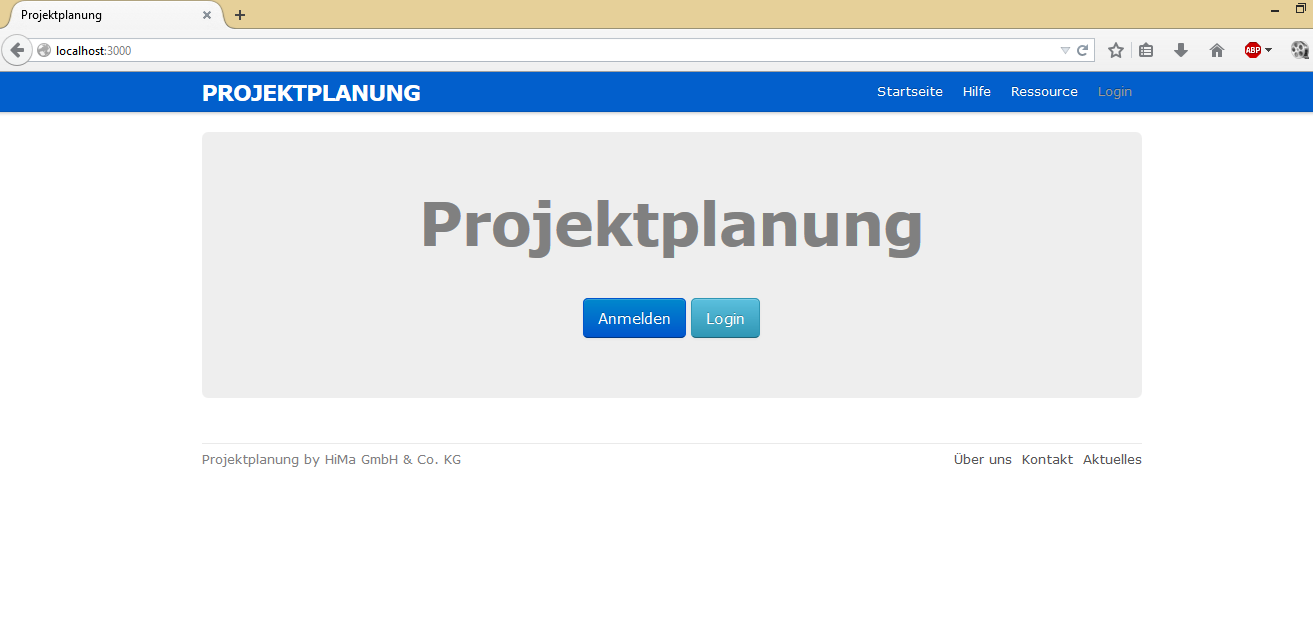
\includegraphics[width=120mm]{Bilder/Startseite_unsigned.png}
    \caption{Startseite Projektplanung Applikation}  \label{Start}
  \end{center}
\end{figure}

Neben Links wie \textit{Hilfe} und \textit{Kontakt} findet sich ein Link \textit{Ressourcen} zur einer Übersicht, in der alle Ressourcen des Projektes gelistet sind. Neben den jeweiligen Ressourcennamen befindet sich ein Button \textit{Bewerben}, der mit der Anmeldeseite verlinkt ist (siehe Abbildung \ref{Anm}). Der Link \textit{Hier geht es zur Anmeldung} führt ebenfalls dorthin. Beschließt sich der Besucher der Seite, sich für das Projekt anzumelden, muss er alle Felder des Anmeldeformulars befüllen.\\

\begin{figure}[h!]
  \begin{center}
    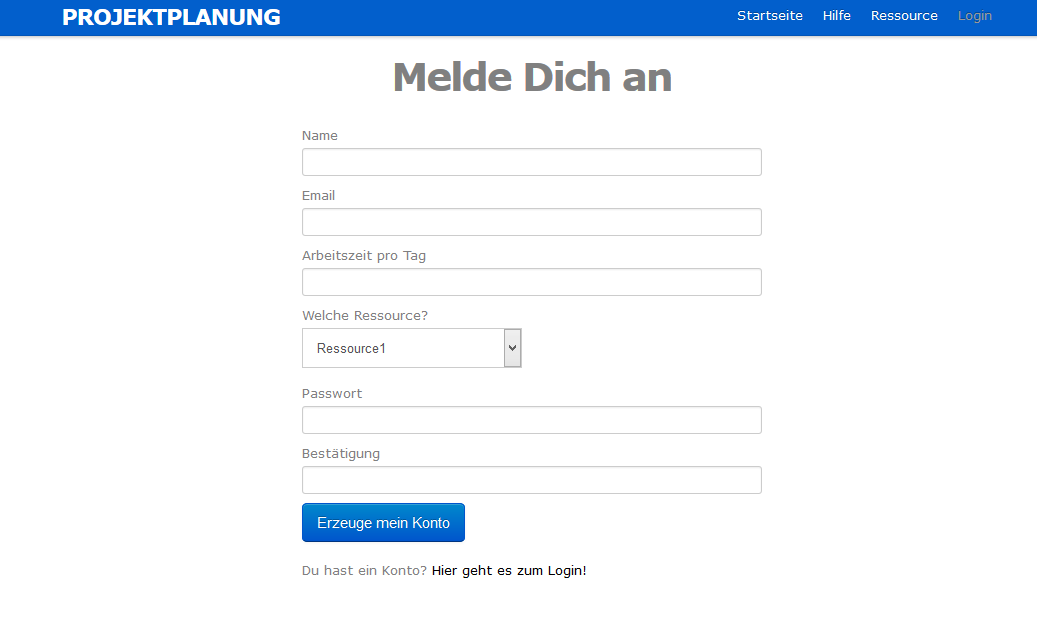
\includegraphics[width=120mm]{Bilder/Anmeldung.png}
    \caption{Anmeldebildschirm}  \label{Anm}
  \end{center}
\end{figure}

Neben dem Namen, einer Mailadresse und eines konformen Passwortes sind projektspezifische Informationen zur erfolgreichen Registrierung nötig. Im Feld \textit{Arbeitszeit pro Tag} muss ein entsprechender Wert eingegeben werden, den der neue User bereit ist, pro Tag für das Projekt an Zeit zu investieren. Wird in diesem Feld keine ganze Zahl, sondern eine Dezimalzahl oder ein Wort eingegeben, kann die Anmeldung im System nicht stattfinden. Es wird ein Fehler angezeigt, der das Defizit aufzeigt und behoben werden muss (siehe Abbildung \ref{Fehler}).\\

\begin{figure}[h!]
  \begin{center}
    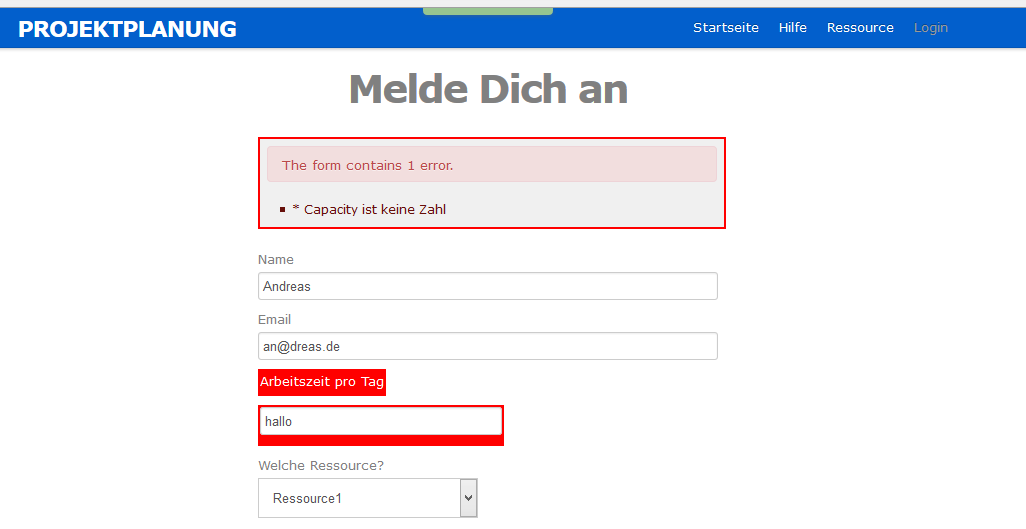
\includegraphics[width=120mm]{Bilder/Anmeldung_Fehleranzeige.png}
    \caption{Fehleranzeige bei Anmeldung}  \label{Fehler}
  \end{center}
\end{figure}

Desweiteren kann eine der vorhandenen Ressourcen ausgewählt werden, in dessen Gruppe der neue Mitarbeiter eingeordnet werden möchte. Findet keine Anmeldung auf der Seite statt, sind keine weiterführenden Tätigkeiten möglich. Die Startseite liefert keine weiterführenden Informationen und bei der Eingabe von anderen Links in die Adresszeile des Browers wird man jederzeit zur \textit{Login}-Seite geführt, da alle Daten für nicht angemeldete Anwender gesperrt sind. Die Verlinkung \textit{"http://localhost:3000/rcpsp/"} öffnet zwar die Seite der Projektplanung, alle angezeigten Buttons führen aber ebenfalls direkt zur Anmeldemaske. \\

Um die Applikation nutzen zu können, ist demzurfolge die Anmeldung als User zwingend notwendig. Findet diese entweder nach erstmaliger Registrierung über den Link \textit{Anmelden} oder über \textit{Login} statt, wird die eigene Profilseite angezeigt (siehe Abbildung \ref{Profil}).\\

\begin{figure}[h!]
  \begin{center}
    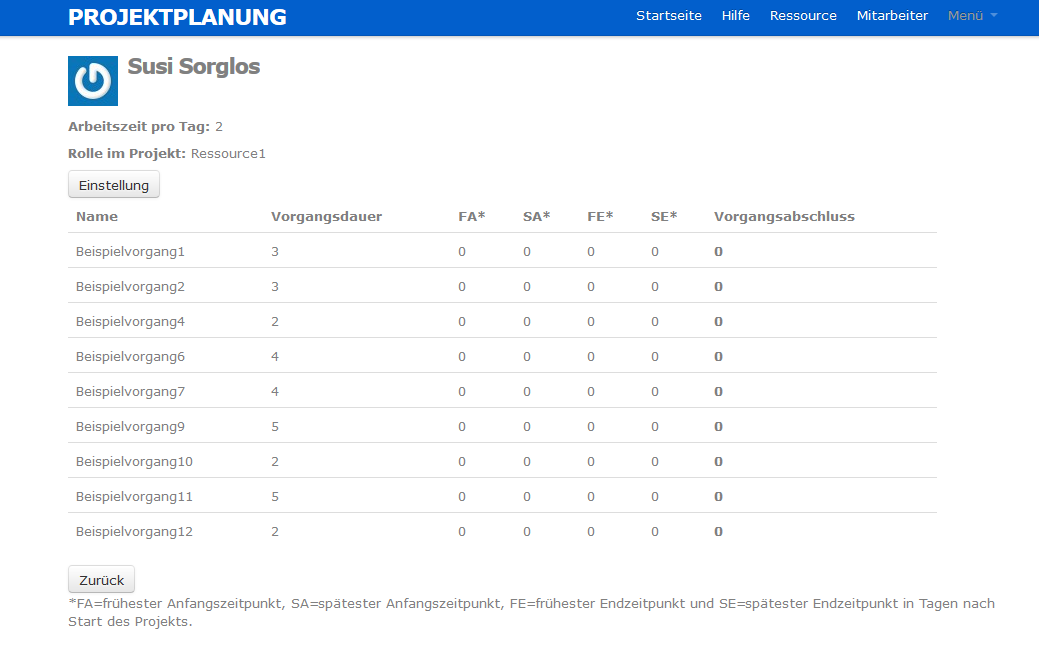
\includegraphics[width=120mm]{Bilder/Profilseite.png}
    \caption{Profilseite eines Users}  \label{Profil}
  \end{center}
\end{figure}

Die Profilseite gibt einen Überblick über all die Daten, die für den User in Hinblick auf das Projekt relevant sind. Es werden die Daten dargestellt, die bei der Anmeldung angegeben wurden (Arbeitszeit, Rolle im Projekt) sowie die Vorgänge, die durch die Wahl der Ressource für diesen User relevant sind, in denen er also arbeiten muss. Zu jedem Vorgang wird die Dauer und gegebenenfalls die Zeitspanne angegeben, wann er jeweils stattfindet. Die Grenze liegt zwischen dem frühesten Startzeitpunkt $FA_{i}$ und spätesten Endzeitpunkt $SE_{i}$ des Vorgangs $i$. Ob diese Tabelle mit Daten gefüllt ist, hängt davon ab, ob das Kapazitäts- bzw. Kostenplanungsproblem bereits gelöst wurde. Möchte der User seine Daten, wie z.B. die Wahl der Ressource oder die Quantität der Arbeitszeit, ändern, gelangt er über den Button \textit{Einstellung} zu einer Seite, die äquivalent aufgebaut ist wie die Anmeldeseite, um dort seine Daten zu aktualisieren. Nach korrekter Eingabe können die Daten über den Button \textit{Speichere Änderungen} gesichert werden. Auf der Profilseite erscheint daraufhin eine Anzeige \textit{"Profil updated"} mit der Bestätigung, dass das Profil aktualisiert wurde. Im Vergleich zum fremden Anwender gelangt der angemeldete User außerdem in der Kopfzeile über den Link \textit{Mitarbeiter} über eine Übersicht aller Mitarbeiter, die für das Projekt auf dieser Applikation angemeldet sind. Die Profilseite jedes Mitarbeiters kann betrachtet werden mit all den Informationen, die auch auf der eigenen Profilseite einzusehen sind. Es können jedoch keine Änderungen vorgenommen werden. Neben der Verlinkung zu der Übersicht der Mitarbeiter lässt sich in der Kopfzeile ein Feld \textit{Menü} finden, dass die Unterpunkte \textit{Profil}, \textit{Einstellungen} und \textit{Logout} enthält. Die Verlinkung \textit{Profil} stellt eine Verlinkung zur Profilseite dar, unter \textit{Einstellungen} kann das eigene Profil aktualisiert werden.\\
Unter \textit{Ressourcen} kann der User, wie auch der nicht angemeldete Anwender, zur Übersicht der vorhandenen Ressourcen gelangen. Die Anzeige stellt sich für den angemeldeten User jedoch vielfältiger dar, als für den einfachen Anwender (siehe Abbildung \ref{ResUs}).\\

\begin{figure}[h!]
  \begin{center}
    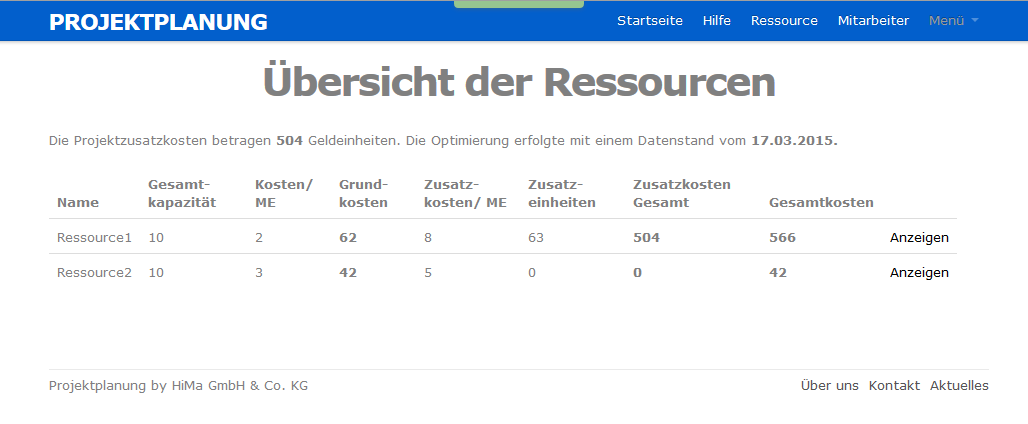
\includegraphics[width=120mm]{Bilder/Ressourcen_User.png}
    \caption{Übersicht der Ressourcen für User}  \label{ResUs}
  \end{center}
\end{figure}

Für den User sind alle Eigenschaften der verschiedenen Ressourcen einsehbar. Es werden die Gesamtkapazität, Kosten pro ME, Grundkosten und Zusatzkosten pro ME angezeigt. Wurde bereits eine Lösung für das Problem der Kostenplanung ermittelt, werden die kalkulierten Werte für die Zusatzeinheiten, gesamten Zusatzkosten und die Gesamtkosten pro Ressource dargestellt. Zudem wird der Zielfunktionswert, bei der Kostenplanung die gesamten anfallenden Zusatzkosten, in Verbindung mit dem Zeitpunkt der Optimierung über der Tabelle dargestellt. Über den Button \textit{Anzeigen} sind die Eigenschaften einer Ressource seperat einsehbar. Da der User bzw. Mitarbeiter in diesem Modell durch die Planung innerhalb des Projektes eingeteilt wird und seine Rechte nicht über die Organisation der eigenen Daten hinaus reicht, hat er keine weiteren Kompetenzen bei der Nutzung dieser Appliaktion. \\

Die Verwaltung der Mitarbeiter und die Organisation sowie Durchführung der Projektplanung kann auschließlich nach der Anmeldung als Administrator erfolgen. Der Admin gilt in dieser Anwendung als durchführende Gewalt, er trägt den Namen \textit{"Example User"}. Nach der erfolgreichen Anmeldung erscheint zunächst erneut die Profilseite, aufgebaut wie beim einfachen User. Im Gegensatz zu normalen Usern bietet die Seite dem Admin jedoch zusätzliche Handlungsspielräume neben der einfachen Auflistung der Vorgänge (siehe Abbildung \ref{ProAd}). Er hat die Möglichkeit, die Dauer der Vorgänge abzuändern oder Vorgänge aus dem Projekt zu löschen. In gleicher Weise stellt sich die Ausweitung der Kompetenzen bei den Ressourcen dar. Über die Verlinkung \textit{Ressourcen} können nun die Ressourcen ebenfalls gelöscht oder die Eigenschaften (Kosten und Zusatzkosten je ME) verändert werden. Desweiteren kann über den Button \textit{Neue Ressource anlegen} eben dies vollzogen werden.\\

\begin{figure}[h!]
  \begin{center}
    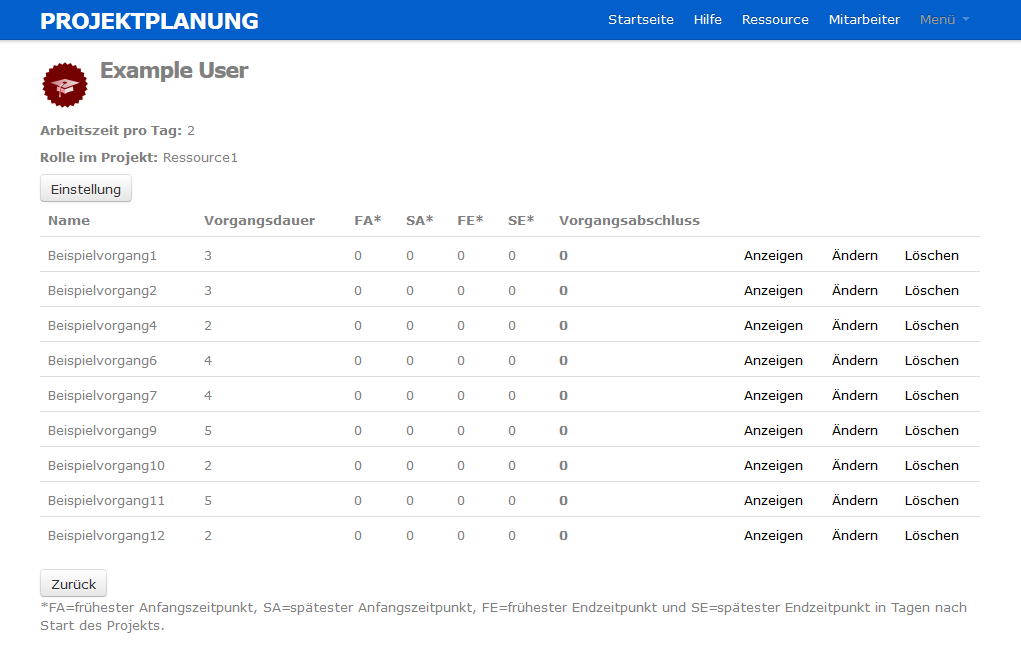
\includegraphics[width=120mm]{Bilder/Profilseite_Admin.png}
    \caption{Profilseite des Administrators}  \label{ProAd}
  \end{center}
\end{figure}             

\begin{figure}[h!]
  \begin{center}
    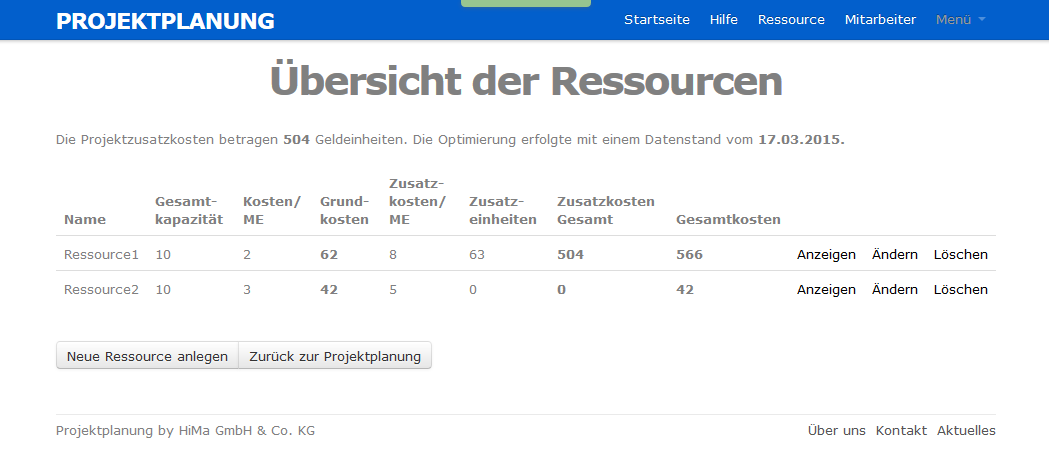
\includegraphics[width=120mm]{Bilder/Ressourcen_Admin.png}
    \caption{Übersicht der Ressourcen aus Sicht des Administrators}  \label{ResAd}
  \end{center}
\end{figure}     
  
Um nun zur Kernaufgabe der Applikation, der Projektplanung, zu gelangen, kann entweder der Button \textit{Zurück zur Projektplanung} getätigt werden, oder in der Kopfzeile wird unter \textit{Menü} der Unterpunkt \textit{Projektplanung} ausgewählt (siehe Abbildung \ref{RCPSP}). Wie bereits erwähnt, hat nur der Admin die Berechtigung, dieses Menü aufzurufen. Im oberen Bereich der Seite sind die Verlinkungen zur Verwaltung der nötigen Inputs zur Lösung beider Planungsproblematiken angesiedelt. Neben den bereits behandelten Links zu den Vorgängen und Ressourcen finden sich Verlinkungen zu den Vorgangsrelationen und Vorgang-Ressourcen-Kombinationen.\\ 

\begin{figure}[h!]
  \begin{center}
    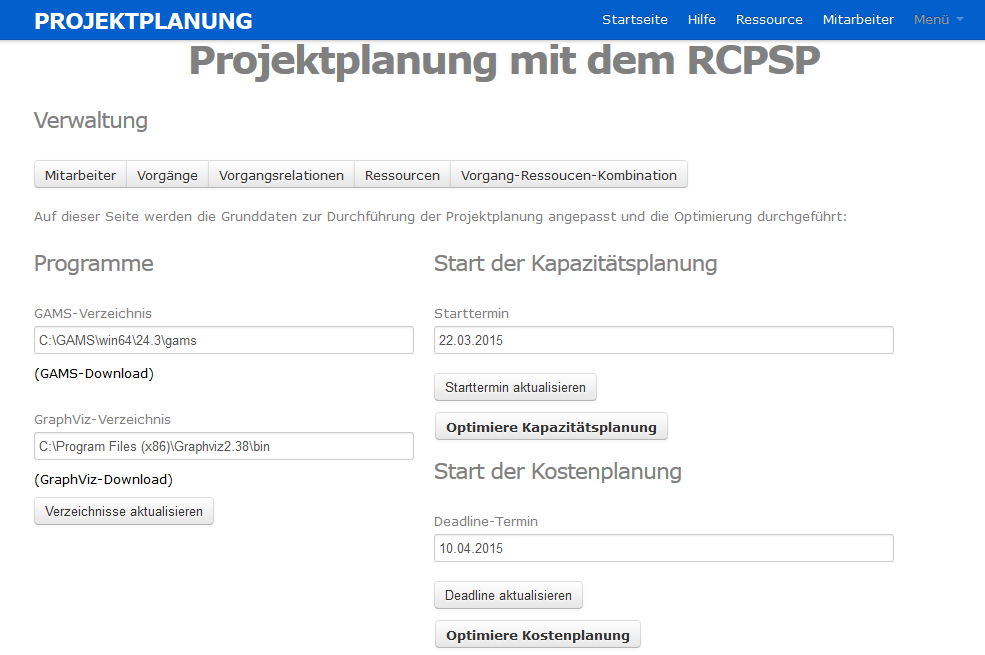
\includegraphics[width=120mm]{Bilder/Projektplanung.png}
    \caption{Projektplanung mit dem RCPSP - Übersicht}  \label{RCPSP}
  \end{center}
\end{figure}

Die Übersicht der Relationen zwischen den Vorgängen stellt eine Auflistung eines jeden Vorgänger und Nachfolger dar. Der Admin kann diese Relationen löschen oder neue anlegen. Wenn er sich dazu entschließt, eine neue anzulegen, ist zu beachten, dass ein Strukturplan eines Projektes keine Zyklen beinhalten darf. Damit Zyklen verhindert werden, findet beim Prozess des Anlegens einer neuen Vorgangsrelation eine Prüfung statt. Beinhaltet die neu angelegte Relation einen Zyklus, tritt ein Fehler auf und die Relationen muss überarbeitet werden (siehe Abbildung \ref{VorErr}). So wird verhindert, dass der Strukturplan Zyklen enthält.\\

\begin{figure}[h!]
  \begin{center}
    
\includegraphics[width=120mm]{Bilder/Vorgangsrel_Fehler.png}
    \caption{Fehler aufgrund eines Zyklus`in der topologischen Reihenfolge}  \label{VorErr}
  \end{center}
\end{figure}
 
Der Button \textit{Vorgang-Ressourcen-Kombination} führt zu einer Übersicht der verschiedenen Ressourcen zu den Vorgängen. Neben der Auflistung können die Kombnationen verändert, gelöscht oder neu erstellt werden. Bei der Veränderung oder Erstellung ist zu beachten,dass die Angabe des Kapazitätsbedarfs nur mit Hilfe einer ganzen Zahl erfolgen darf. Entsprechend der Kapazitätsangabe bei der Bearbeitung eines Profils erscheint bei jeder anderen Art von Eingabe ein Fehler, der die Datenspeicherung verhindert.\\
Nachdem all diese Daten geprüft und gegebenfalls verändert wurden, steht die Basis sowohl für die Optimierung der Kapazitäts- als auch der Kostenplanung. Bevor der Optimierungsprozess stattfinden kann, müssen noch einige Rahmenbedingungen geprüft werden. Da die Optimierung mit dem Programm \textit{GAMS} stattfindet, muss die Applikation auf dieses Programm zurückgreifen können. Dafür muss \textit{GAMS} auf dem hiesigen Computer installiert sein. Nach der Recherche des Installationsortes muss der korrekte Pfad in das Feld eingetragen werden, in dem der Beispielpfad zu sehen ist. Nach der Eingabe wird der Pfadzugriff durch \textit{Verzeichnis aktualisieren} eingestellt (siehe Abbildung \ref{RCPSP}).


     


%\lstinputlisting[language=ruby, firstline=37, lastline=45, caption=Name, style=Listing]{Dateiname.html}



\section{Kritische Würdigung des Anwendungssystems} \label{krit}

\section{Fazit} \label{Fazit}

\bibliographystyle{Prod_Seminar}    %legt die zu verwendende BIBTEX-Stildatei fest
\newpage
\bibliography{Literatur}    %an der Stelle zu verwenden, an der das Literaturverzeichnis gesetzt werden soll;
                            %Literatur ist der Dateiname der BIB-Datei mit den LiteraturLiteratur-Informationen

\newpage
%%%%%%%%%%%%%%%%%%%%%%%%%%%%%%%%%%%%%%%%%%%%%%%%%%%%%%
%
%    ggf. Anhang
%
%%%%%%%%%%%%%%%%%%%%%%%%%%%%%%%%%%%%%%%%%%%%%%%%%%%%%%
\begin{appendix}
\section{Anhang}

\subsection{GAMS-Implementierung des Beispiels}\label{Imp}

\subsection{Ruby on Rails Programmcode}\label{Anhang2}


\end{appendix}
\end{document}
%%%%%%%%%%%%%%%%%%%%%%%%%%ENDE%%%%%%%%%%%%%%%%%%%

